\documentclass[10pt,a4paper]{article}
\usepackage[margin=17mm]{geometry}
\usepackage{graphicx,booktabs,hyperref}
\pagestyle{empty}
\begin{document}
\noindent{\Large\bfseries Canonical-row scan: production integration}\\[3pt]
{\small Rust, 27 November 2026. PR \#5251. Runtime benefit unmeasured.}
\paragraph{Change.} Both native certificate checkers now use a read-only row-form scan on the bounded uncounted path. The same comparator checks strict order; coefficients must be canonical/nonzero. Empty or nonmonic rejection, input reductions, all pair/graph obligations and original-ideal proof checks remain. Active Visit or bitop accounting and unsupported shapes keep the original normalization path. The public normalizer is unchanged.
\begin{center}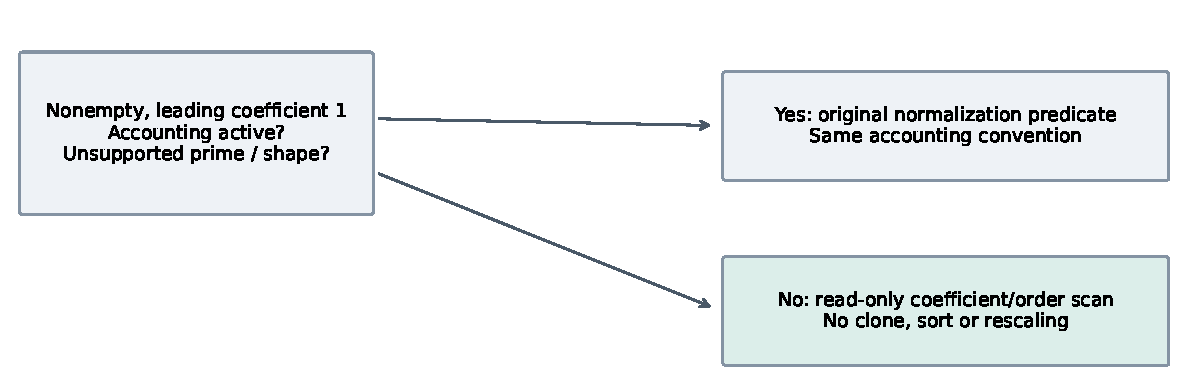
\includegraphics[width=\linewidth]{canonical-check.pdf}\end{center}
\noindent Fast domain: primes 2147483647/9007199254740881, uniform 3..16-variable rows, exponents$\leq64$. No new selection seed or performance input is introduced.
\paragraph{Qualification.} Three candidate unit functions pass on 15804 differential rows against actual production normalization plus branch/fallback tests. A fourth unit imports the live production file directly and passes 31500 comparisons under both accounting flags. In the tested monic row, the uncounted helper makes zero normalization calls; the accounted helper makes one. No runtime is inferred from that operation check. [pcc:unverified]
\begin{center}\begin{tabular}{lr}\toprule
Scope & Recorded outcome\\\midrule
Old/new fixed matrices &432 cases each\\
Complete public reverification &432 per matrix\\
Exact matrix payload parity &1729 files identical\\
Native original / matched cases &36 /108 pass\\
Mutation assertions / unsupported refusals &1116 /6\\
Complete separate native proof audits &144 proofs;2+5 canaries refused\\
Native output parity &181 /433 files identical\\\bottomrule\end{tabular}\end{center}
\noindent Both bitop-disabled and enabled modes are covered. Every complete proof, basis, native receipt and enabled per-phase primitive count matches the baseline byte for byte. Source and actual root builds are pinned; the promoted helper equals the qualified candidate. All results are unsigned same-host evidence. [pcc:unverified]
\paragraph{Limits.} No separate full Visit-ledger campaign or optimized performance build was qualified. Counted calls retain legacy normalization, so no frozen cost-model credit is booked. Prior whole-libtest allocation failures remain historical. Baseline raw exits are 0 while the outer observer reports 1; both observations remain retained, with no silent rerun. Candidate/native/auditor captured exits are 0; the additional live unit also has raw0/outer1, retained separately. [pcc:unverified]
\paragraph{Next.} No comparative timing ran; 15$\times$ remains unachieved, and intrinsic regularity/F4 solving degree remain unknown. Canonical timing-document choice is pending; Conductor and checkpoint/S3 are waived. A future campaign must retain old root pair-graph arms as eligible controls and qualify both new native versions, with the original full boundary, repetitions/A/A, six fixed inputs and every proof/failure gate.
\paragraph{Reproduce.} README, PLAN/INTEGRATION\_PLAN, separate source/pre-call records, complete old/new matrices and native cohorts, six immutable workers plus the live-unit worker, raw logs and source preimages are supplied. The report only renders recorded values.
\end{document}
